\chapter{Implementacija i korisničko sučelje}
		
		
		\section{Korištene tehnologije i alati}
		
			\textbf{\textit{dio 2. revizije}}
			
			 \textit{Detaljno navesti sve tehnologije i alate koji su primijenjeni pri izradi dokumentacije i aplikacije. Ukratko ih opisati, te navesti njihovo značenje i mjesto primjene. Za svaki navedeni alat i tehnologiju je potrebno \textbf{navesti internet poveznicu} gdje se mogu preuzeti ili više saznati o njima}.
			
			
			\eject 
		
	
		\section{Ispitivanje programskog rješenja}
			
Nakon što smo završili s izradom testirali smo rad aplikacije koristeći JUnit tehnologiju i
Selenium WebDriver. Testovi su dali zadovoljavajuće rezultate te možemo zaključiti da smo uspjeli implementirati zadane funkcionalnosti.
			
			\subsection{Ispitivanje komponenti}
			
Za ispitivanje komponenti koristili smo JUnit tehnologiju. JUnit okvir je za testiranje komponenti sustava programiranog u Javi. Ispitali smo funkcionalnosti ažuriranja osobnih podataka donora, promjenu optimalnih granica krvi i evidencije krvi slanjem u instituciju. Koriste se objekti tipa UserContoller, BloodController i ConsumptionController na kojima se pozivaju ispitivane funkcionalnosti te UserService, BloodService i RoleService koji su potrebni za dohvaćanje podataka korištenih u funkcijama.
\\\\
\textbf{Ažuriranje osobnih podataka donora}
\\\\
Pozivom funkcije getEditUserInfo iz klase UserController želimo donoru uspješno promijeniti prezime. Na kraju uspoređujemo je li prezime ažuriranog donora jednako željenom novom prezimenu.
\\\\
\begin{figure}[H]
	\centering
	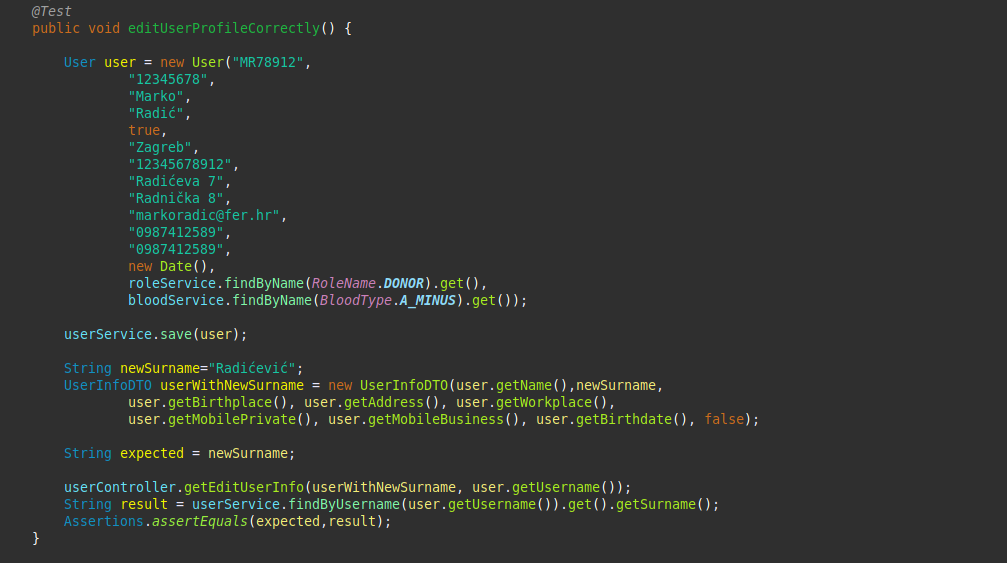
\includegraphics[width=\textwidth, scale=0.5]{dijagrami/unit1}
	\caption{Unit test1}
\end{figure}
	
U idućem testu pozivom iste funkcije želimo neuspješno ažurirati polje rejected, koje se ne bi smjelo mijenjati. Na kraju uspoređujemo je li dobivena statusn poruka jednaka očekivanoj "400" što bi značilo da aplikacija na pobuđeno situaciju prikladno odgovara.

	
			
			
			\subsection{Ispitivanje sustava}
			
			 \textit{Potrebno je provesti i opisati ispitivanje sustava koristeći radni okvir Selenium\footnote{\url{https://www.seleniumhq.org/}}. Razraditi \textbf{minimalno 4 ispitna slučaja} u kojima će se ispitati redovni slučajevi, rubni uvjeti te poziv funkcionalnosti koja nije implementirana/izaziva pogrešku kako bi se vidjelo na koji način sustav reagira kada nešto nije u potpunosti ostvareno. Ispitni slučaj se treba sastojati od ulaza (npr. korisničko ime i lozinka), očekivanog izlaza ili rezultata, koraka ispitivanja i dobivenog izlaza ili rezultata.\\ }
			 
			 \textit{Izradu ispitnih slučajeva pomoću radnog okvira Selenium moguće je provesti pomoću jednog od sljedeća dva alata:}
			 \begin{itemize}
			 	\item \textit{dodatak za preglednik \textbf{Selenium IDE} - snimanje korisnikovih akcija radi automatskog ponavljanja ispita	}
			 	\item \textit{\textbf{Selenium WebDriver} - podrška za pisanje ispita u jezicima Java, C\#, PHP koristeći posebno programsko sučelje.}
			 \end{itemize}
		 	\textit{Detalji o korištenju alata Selenium bit će prikazani na posebnom predavanju tijekom semestra.}
			
			\eject 
		
		
		\section{Dijagram razmještaja}
			
			Dijagrami razmještaja prikazuju topologiju sustava i odnos sklopovskih i program-
skih dijelova. Olakšavaju nam vizualizaciju razmještaja fizičkog dijela sustava i
sklopovlja. Sustav se sastoji od klijentskog i poslužiteljskog računala. Klijent na
svojem računalu preko web preglednika pristupa aplikaciji. Klijentsko računalo
komunicira s poslužiteljskim računalom preko HTTP veze. Na poslužiteljskom se
računalu nalaze web poslužitelj i poslužitelj baze podataka (PostgreSQL).

\begin{figure}[H]
	\centering
	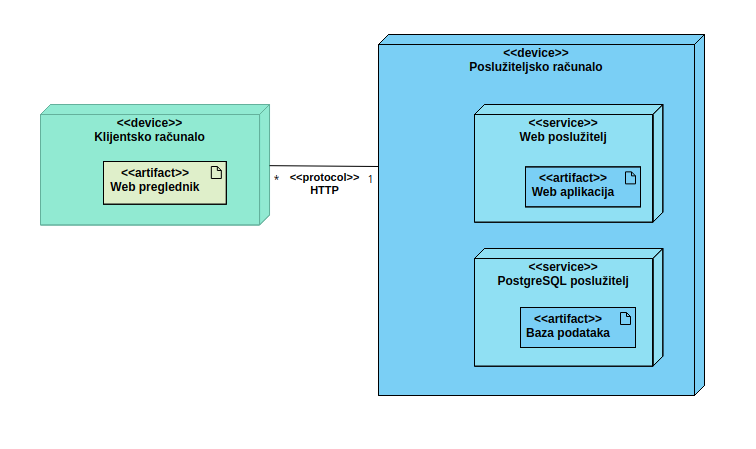
\includegraphics[width=\textwidth, scale=0.5]{dijagrami/dijagram_razmjestaja}
	\caption{Dijagram razmještaja}
	\label{fig:dijagram_razmještaja}
\end{figure}
			
			
			\eject 
		
		\section{Upute za puštanje u pogon}
		
			\textbf{\textit{dio 2. revizije}}\\
		
			 \textit{U ovom poglavlju potrebno je dati upute za puštanje u pogon (engl. deployment) ostvarene aplikacije. Na primjer, za web aplikacije, opisati postupak kojim se od izvornog kôda dolazi do potpuno postavljene baze podataka i poslužitelja koji odgovara na upite korisnika. Za mobilnu aplikaciju, postupak kojim se aplikacija izgradi, te postavi na neku od trgovina. Za stolnu (engl. desktop) aplikaciju, postupak kojim se aplikacija instalira na računalo. Ukoliko mobilne i stolne aplikacije komuniciraju s poslužiteljem i/ili bazom podataka, opisati i postupak njihovog postavljanja. Pri izradi uputa preporučuje se \textbf{naglasiti korake instalacije uporabom natuknica} te koristiti što je više moguće \textbf{slike ekrana} (engl. screenshots) kako bi upute bile jasne i jednostavne za slijediti.}
			
			
			 \textit{Dovršenu aplikaciju potrebno je pokrenuti na javno dostupnom poslužitelju. Studentima se preporuča korištenje neke od sljedećih besplatnih usluga: \href{https://aws.amazon.com/}{Amazon AWS}, \href{https://azure.microsoft.com/en-us/}{Microsoft Azure} ili \href{https://www.heroku.com/}{Heroku}. Mobilne aplikacije trebaju biti objavljene na F-Droid, Google Play ili Amazon App trgovini.}
			
			
			\eject 